% arara: pdflatex: { shell: yes }
\documentclass{article}
\usepackage[utf8]{inputenc}
\usepackage{array}
\usepackage{hyperref}
\usepackage{float}
\usepackage{graphicx}
\bibliographystyle{apacite}

% Suppress underfull and overfull warnings
\hbadness=10000
\hfuzz=10000pt

\begin{document}

\title{Object-relational database}
\author{Erick Gonzalez Parada 178145\\
    Antonio Gutiérrez Blanco 177442\\
    Andre Francois Duhamel Gutierrez 177315\\
    Emiliano Ruiz Plancarte 177478\\ }
\date{\today}

\maketitle

\section{Objective}
\begin{sloppypar}
To design, implement, and evaluate an object-relational database system by defining complex object types, creating relational tables with nested collections, and establishing relationships between objects. The goal is to demonstrate the effective use of Object Query Language (OQL) for managing object-relational data structures, inserting sample data, and performing queries to validate the schema's functionality and integrity.
\end{sloppypar}

\section{Introduction}

\vspace{1cm}

{\Huge{ There is an EXTRA section at the end, please don't forget}}

\vspace{1cm}
Object Query Language (OQL) is a standardized query language designed for querying and manipulating object-oriented databases. Unlike traditional SQL, which is tailored for relational databases, OQL is specifically built to handle complex object-oriented data structures, such as inheritance, polymorphism, and nested collections. OQL allows developers to interact with object-relational databases in a way that aligns with the principles of object-oriented programming, making it a powerful tool for modern database systems\cite{ibm}.
\\
OQL revolves around its ability to query objects and their relationships directly, rather than relying on flat, tabular structures. This is particularly useful in scenarios where data is represented as objects with attributes, methods, and relationships to other objects\cite{mendix}.

\section{Literature Review}

Traditional SQL (Structured Query Language) is designed for relational databases, where data is stored in flat, tabular structures. The philosophy of SQL revolves around the use of \textbf{joins} to combine data from multiple tables, enabling users to retrieve related information. For example, to retrieve data about an employee and their department, SQL requires joining the \texttt{Employee} and \texttt{Department} tables using a common key. While this approach is effective for relational data, it becomes cumbersome and inefficient when dealing with complex, hierarchical, or object-oriented data structures\cite{w3s}.

In contrast, Object Query Language (OQL) is specifically designed for object-oriented databases, where data is represented as objects with attributes, methods, and relationships. OQL eliminates the need for explicit joins by allowing developers to \textbf{directly traverse object relationships}. For instance, in an object-relational database, an \texttt{Employee} object might have a direct reference to a \texttt{Department} object. With OQL, querying the department of an employee is as simple as navigating the object hierarchy (e.g., \texttt{employee.department}), without the need for complex joins or intermediate tables\cite{mendix}.

While SQL can simulate some object-oriented behavior---such as using foreign keys and nested queries to represent relationships---it lacks the native support for object-oriented principles like \textbf{inheritance}, \textbf{polymorphism}, and \textbf{nested collections}. For example, simulating inheritance in SQL requires creating multiple tables and using complex joins to represent parent-child relationships. Similarly, representing nested collections (e.g., a list of phone numbers for an employee) often involves creating additional tables and performing multiple joins, which can lead to inefficient queries and increased complexity\cite{ibm}.

OQL, on the other hand, natively supports these object-oriented features. It allows developers to define \textbf{complex object types}, \textbf{inheritance hierarchies}, and \textbf{nested collections} directly in the database schema. This makes OQL more intuitive and efficient for querying object-oriented data, as it aligns with the natural structure of the data. For example, querying a nested collection of phone numbers in OQL is straightforward (e.g., \texttt{employee.phones}), whereas in SQL, it requires joining multiple tables and aggregating results\cite{mendix}.

In summary, while SQL remains a powerful tool for relational data, its reliance on joins and lack of native support for object-oriented principles make it less suitable for modern, object-oriented applications. OQL addresses these limitations by providing a query language that is inherently designed for object-relational databases, enabling more efficient and intuitive data retrieval and manipulation.

\section{Methodology}
To implement and evaluate the object-relational database system, we used \textbf{Oracle Database Express Edition (XE)} as the primary database management system. The general solution involved the following steps:

1. \textbf{Setting Up Oracle Database Express}:
   - Oracle Database XE was downloaded and installed on a local machine. During installation, the default settings were used, and a system password was set for the administrative user (\texttt{SYS}).
   - The database was configured to allow remote connections, and the necessary ports (e.g., 1521 for Oracle) were opened to enable access from external tools.

2. \textbf{Configuring Visual Studio Code (VSCode)}:
   - The \textbf{Oracle Developer Tools for VSCode} extension was installed to facilitate database connectivity and query execution.
   - A connection profile was created in VSCode, specifying the host (e.g., \texttt{localhost}), port (e.g., \texttt{1521}), service name (e.g., \texttt{XE}), and credentials (e.g., \texttt{SYS} and the system password).

	 \begin{figure}[H]
		 \centering
		 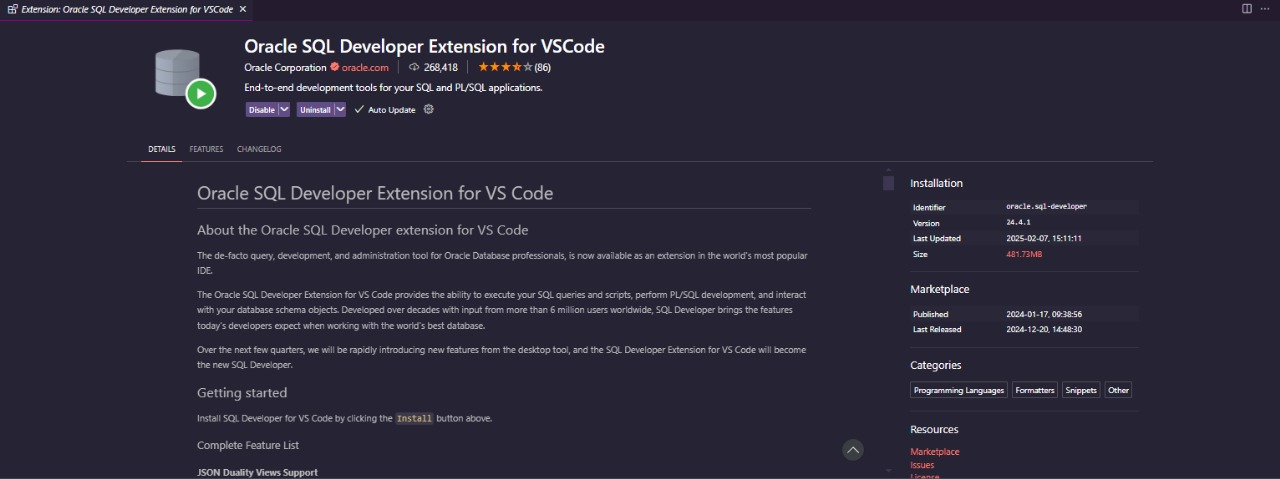
\includegraphics[width=1\textwidth]{imgs/ext.jpeg}
		 \caption{VSCode extension}
		 \label{fig:1}
		\end{figure}

3. \textbf{Writing and Executing OQL Scripts}:
   - OQL scripts were written to define complex object types, create relational tables with nested collections, and establish relationships between objects. These scripts were saved as \texttt{.sql} files for execution.
   - The scripts included:
     - \textbf{Object Type Definitions}: Creating object types such as \texttt{employee\_t}, \texttt{worker\_t}, and \texttt{manager\_t} with attributes and methods.
     - \textbf{Table Creation}: Defining tables with nested collections (e.g., \texttt{telephone\_t} as a nested table of phone numbers).
     - \textbf{Data Insertion}: Inserting sample data into the tables to populate the database.
     - \textbf{Query Execution}: Writing and executing queries to retrieve and validate data from the object-relational schema.

4. \textbf{Challenges Faced}:
   - One of the major challenges was the \textbf{lack of comprehensive online documentation} for OQL, especially in the context of Oracle Database. This made it difficult to troubleshoot issues and find examples of advanced OQL features.
   - Additionally, configuring the Oracle extension in VSCode required trial and error, as some settings (e.g., connection parameters) were not well-documented.

5. \textbf{Validation and Testing}:
   - After executing the OQL scripts, the database schema and data were validated by running queries to ensure that object relationships, nested collections, and inheritance hierarchies were functioning as expected.
   - The results were compared with the expected outcomes to verify the correctness and efficiency of the implemented schema.

\section{Result Analysis}
The following figures will show us the whole work done for our solution and how the oql compiled successfully:

\begin{figure}[H]
	\centering
	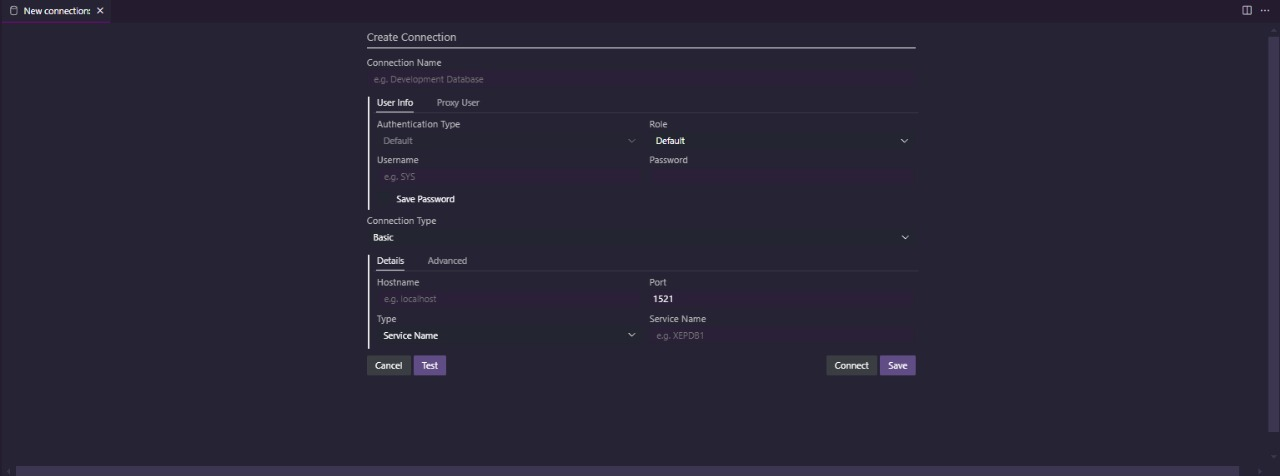
\includegraphics[width=1\textwidth]{imgs/cconn.jpeg}
	\caption{Create connection}
	\label{fig:2}
\end{figure}

\begin{figure}[H]
	\centering
	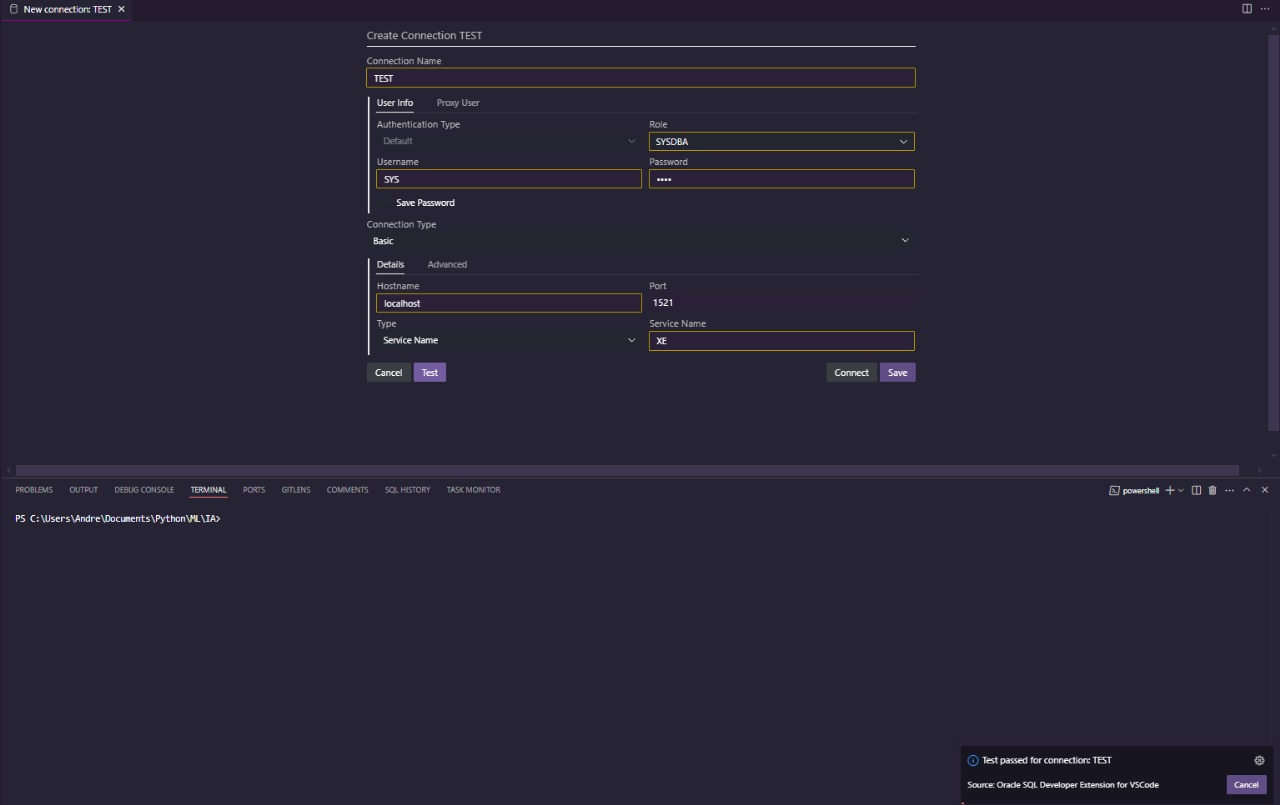
\includegraphics[width=1\textwidth]{imgs/setConn.jpeg}
	\caption{Setting connection}
	\label{fig:3}
\end{figure}

\begin{figure}[H]
	\centering
	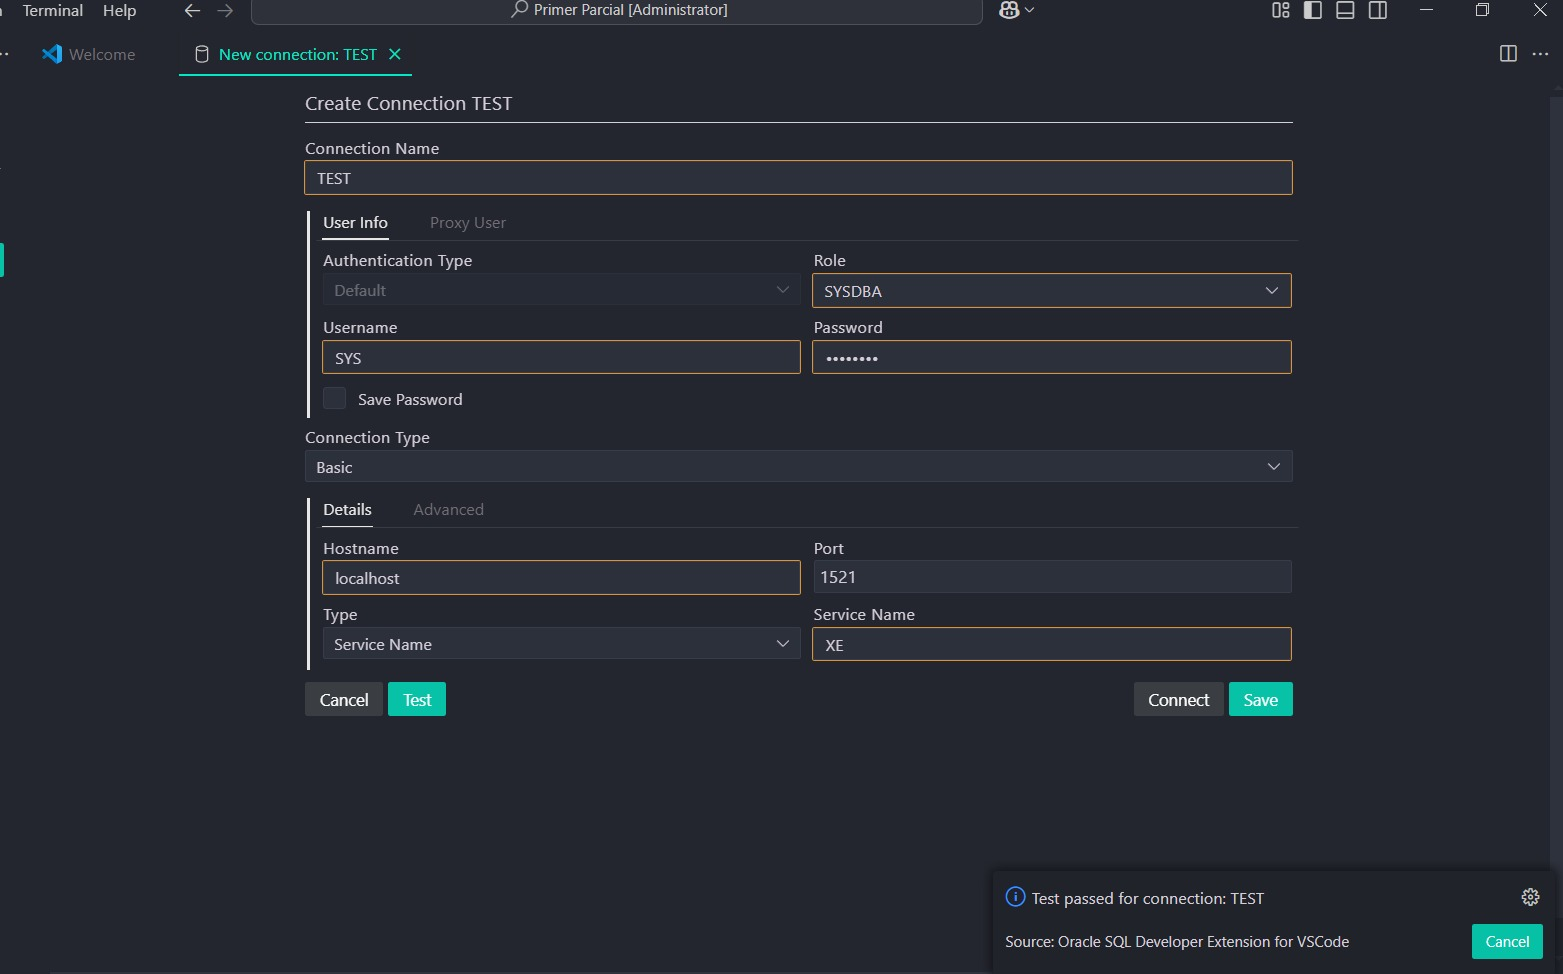
\includegraphics[width=1\textwidth]{imgs/setConn2.jpeg}
	\caption{Setting connection}
	\label{fig:4}
\end{figure}

\begin{figure}[H]
	\centering
	
\includegraphics[width=1\textwidth]{imgs/selConn.jpeg}
	\caption{Connection selection}
	\label{fig:5}
\end{figure}

\begin{figure}[H]
	\centering
	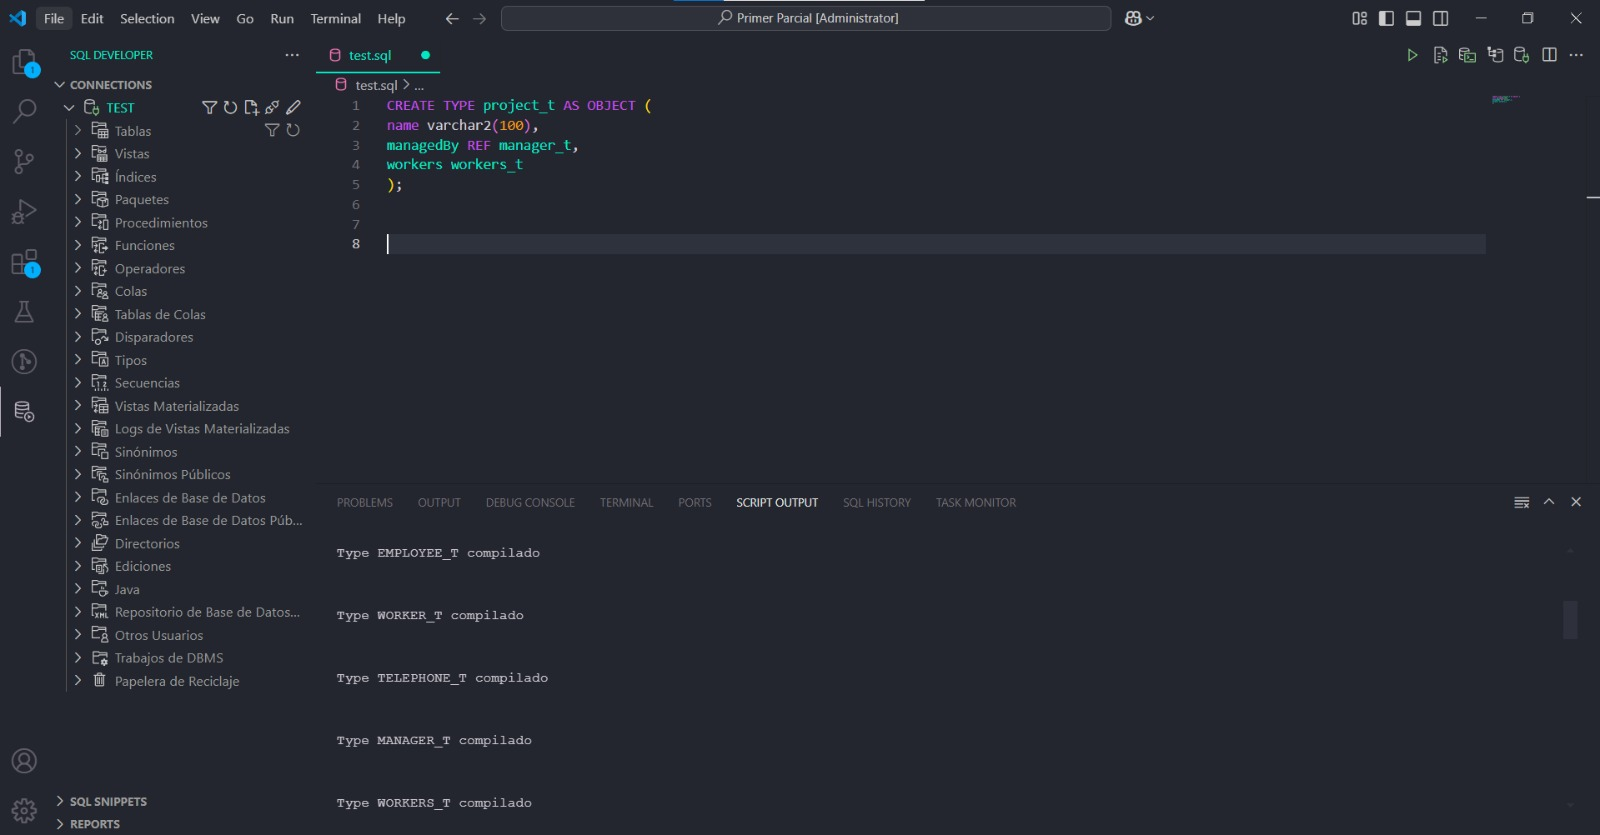
\includegraphics[width=1\textwidth]{imgs/c1.jpeg}
	\caption{Create query}
	\label{fig:6}
\end{figure}

\begin{figure}[H]
	\centering
	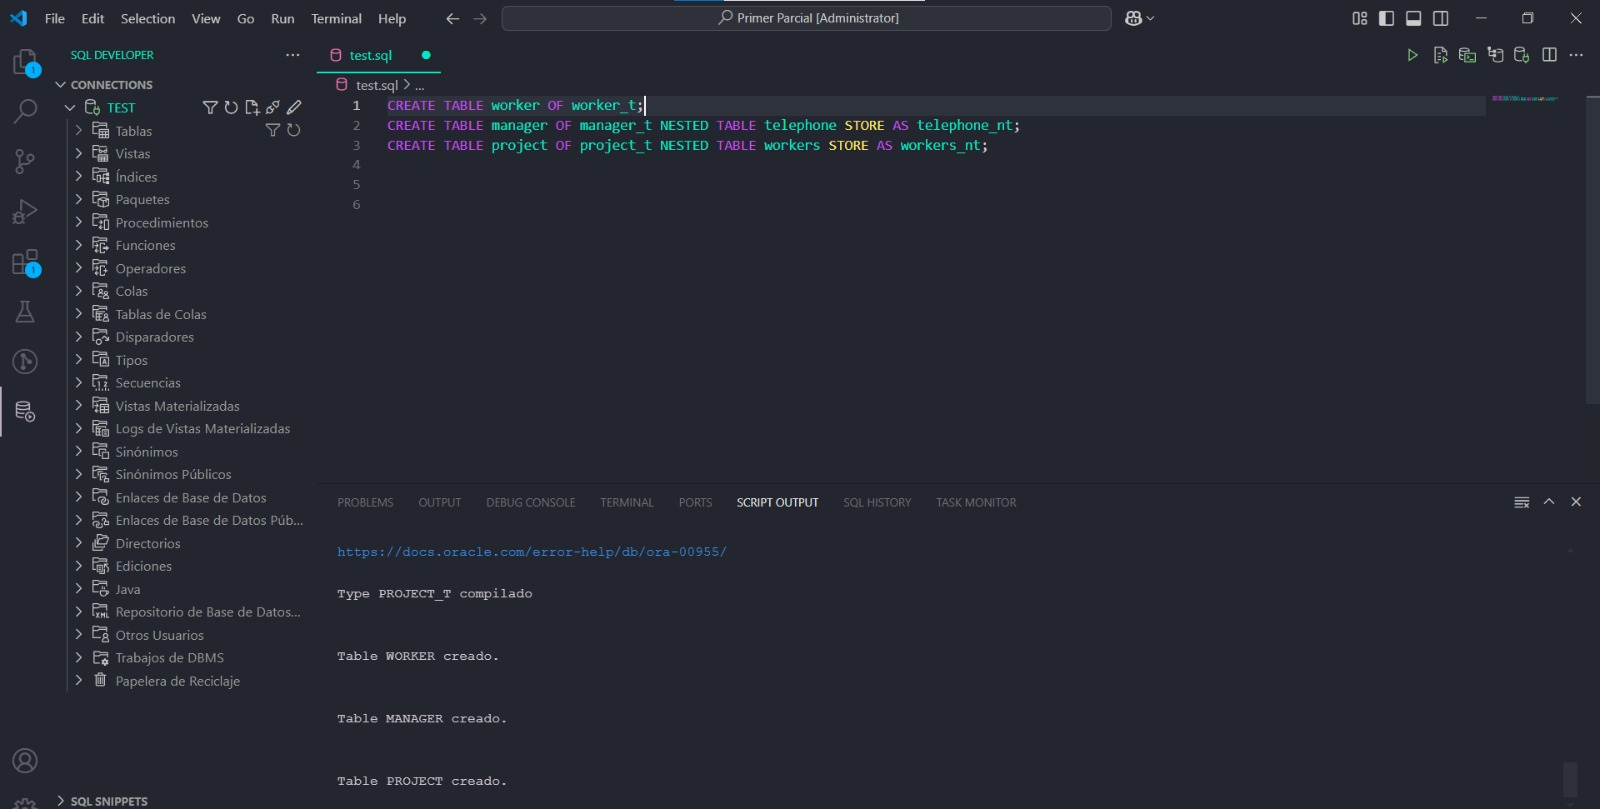
\includegraphics[width=1\textwidth]{imgs/c2.jpeg}
	\caption{Create query}
	\label{fig:7}
\end{figure}

\begin{figure}[H]
	\centering
	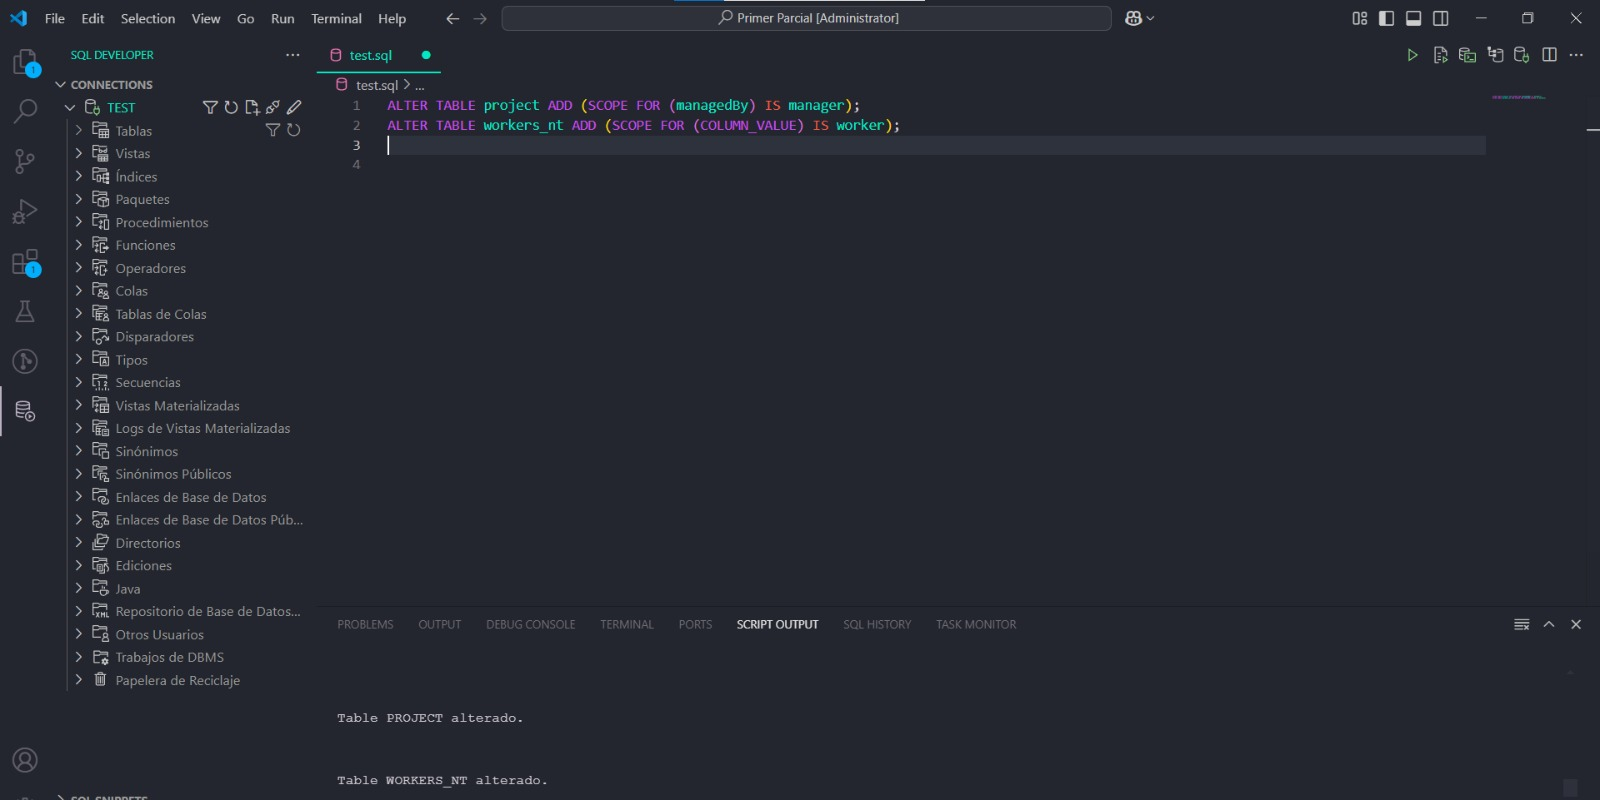
\includegraphics[width=1\textwidth]{imgs/al.jpeg}
	\caption{Alter query}
	\label{fig:8}
\end{figure}

\begin{figure}[H]
	\centering
	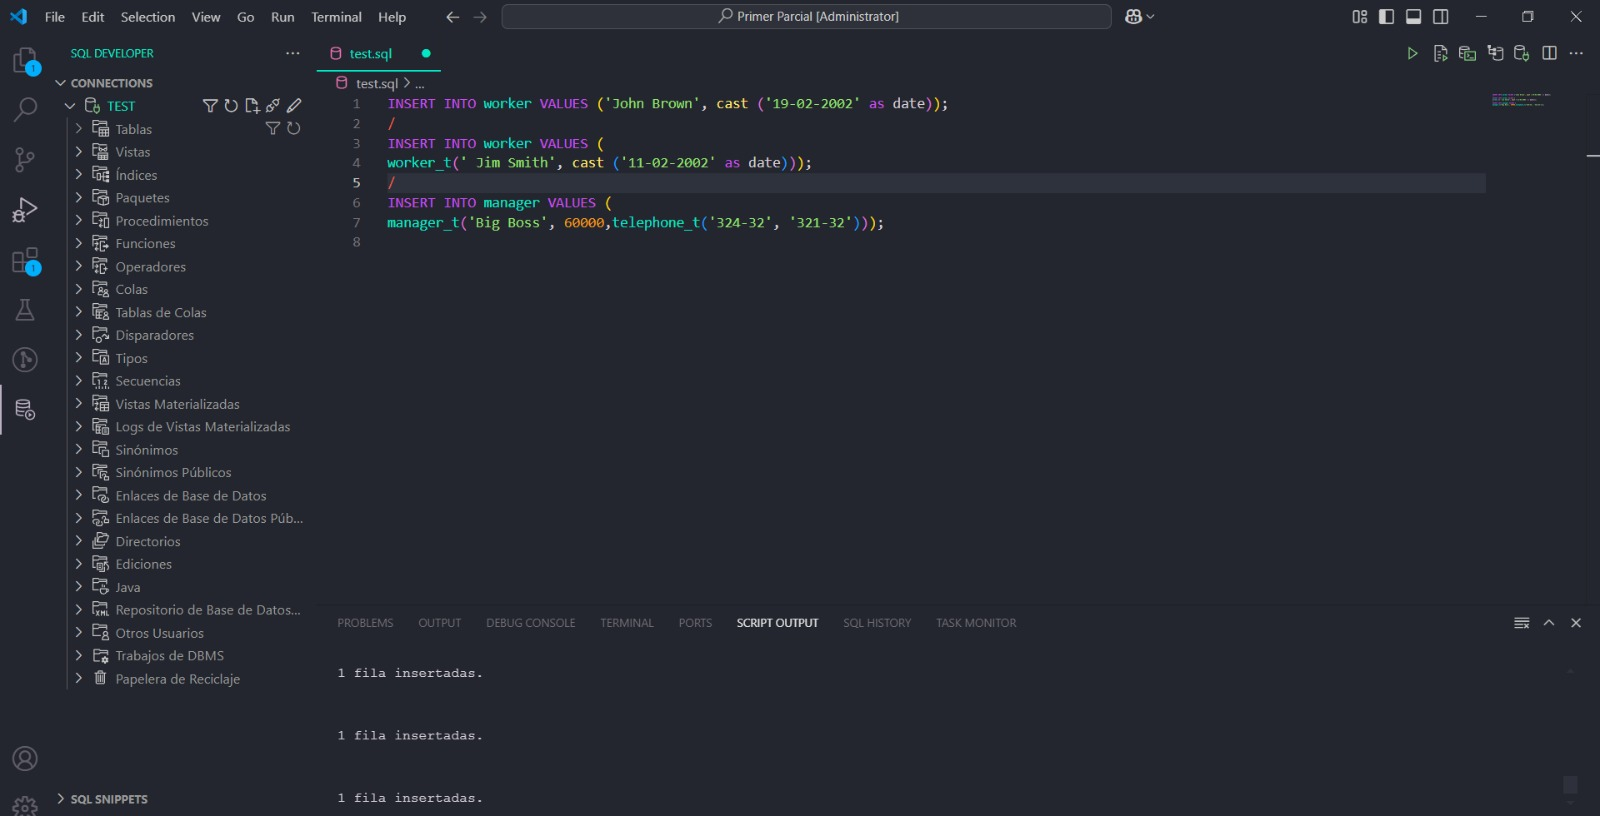
\includegraphics[width=1\textwidth]{imgs/inse1.jpeg}
	\caption{Insert query}
	\label{fig:9}
\end{figure}

\begin{figure}[H]
	\centering
	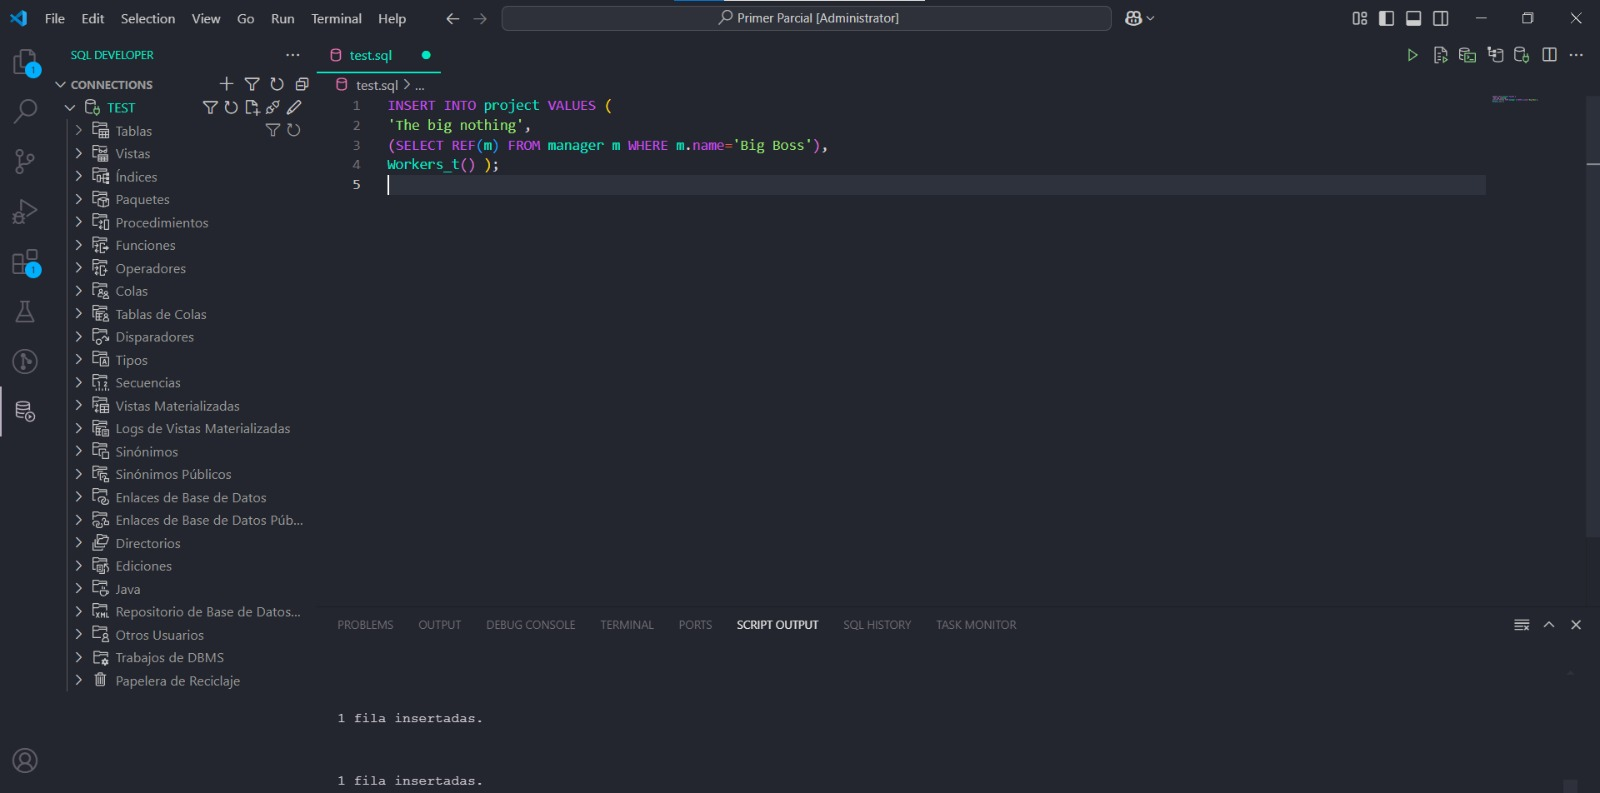
\includegraphics[width=1\textwidth]{imgs/inse2.jpeg}
	\caption{Insert query}
	\label{fig:10}
\end{figure}

\begin{figure}[H]
	\centering
	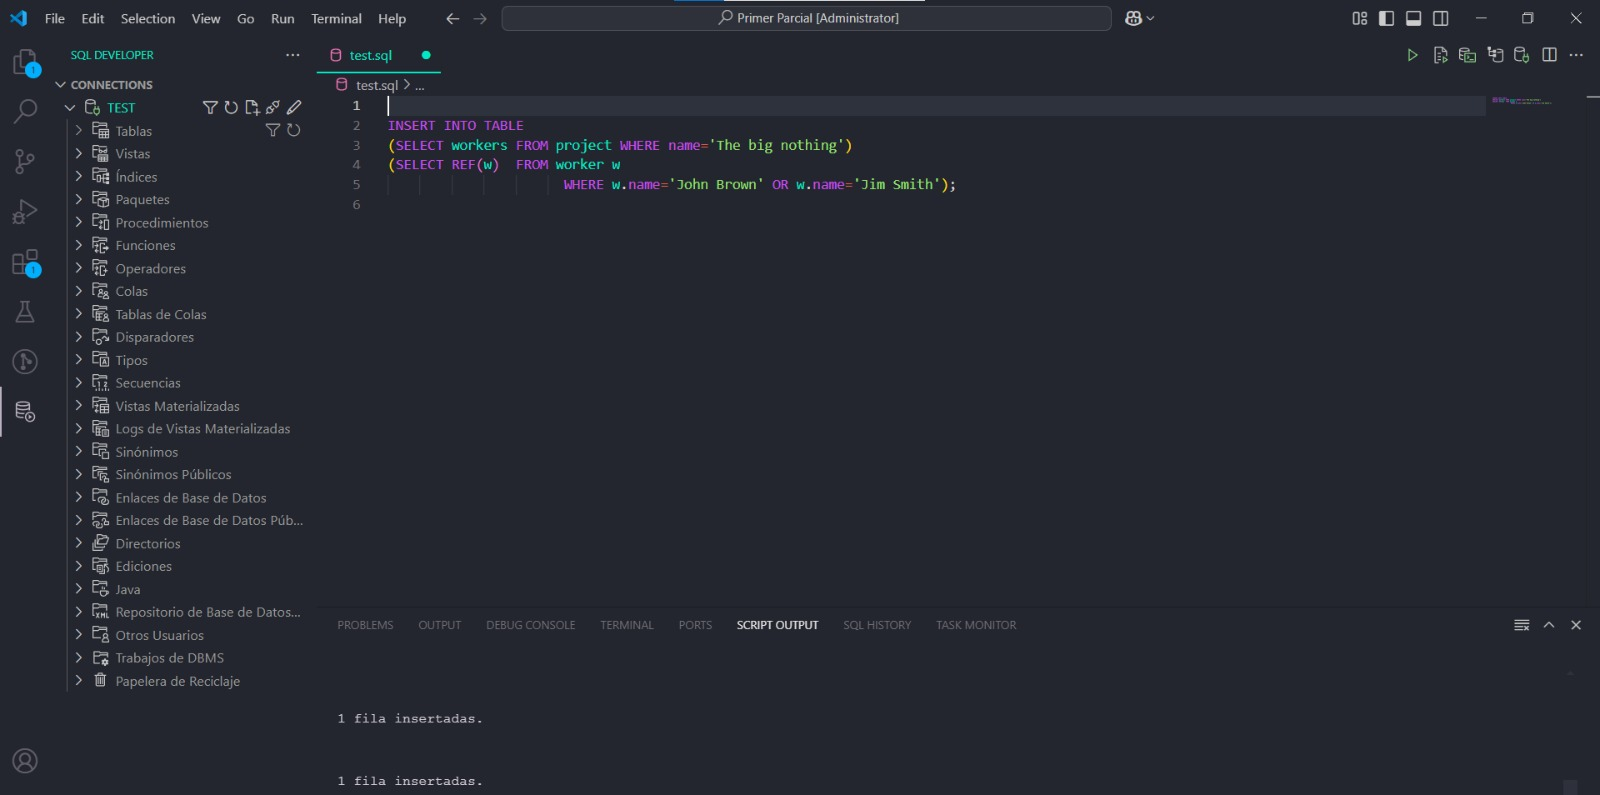
\includegraphics[width=1\textwidth]{imgs/inse3.jpeg}
	\caption{Insert query}
	\label{fig:11}
\end{figure}

\begin{figure}[H]
	\centering
	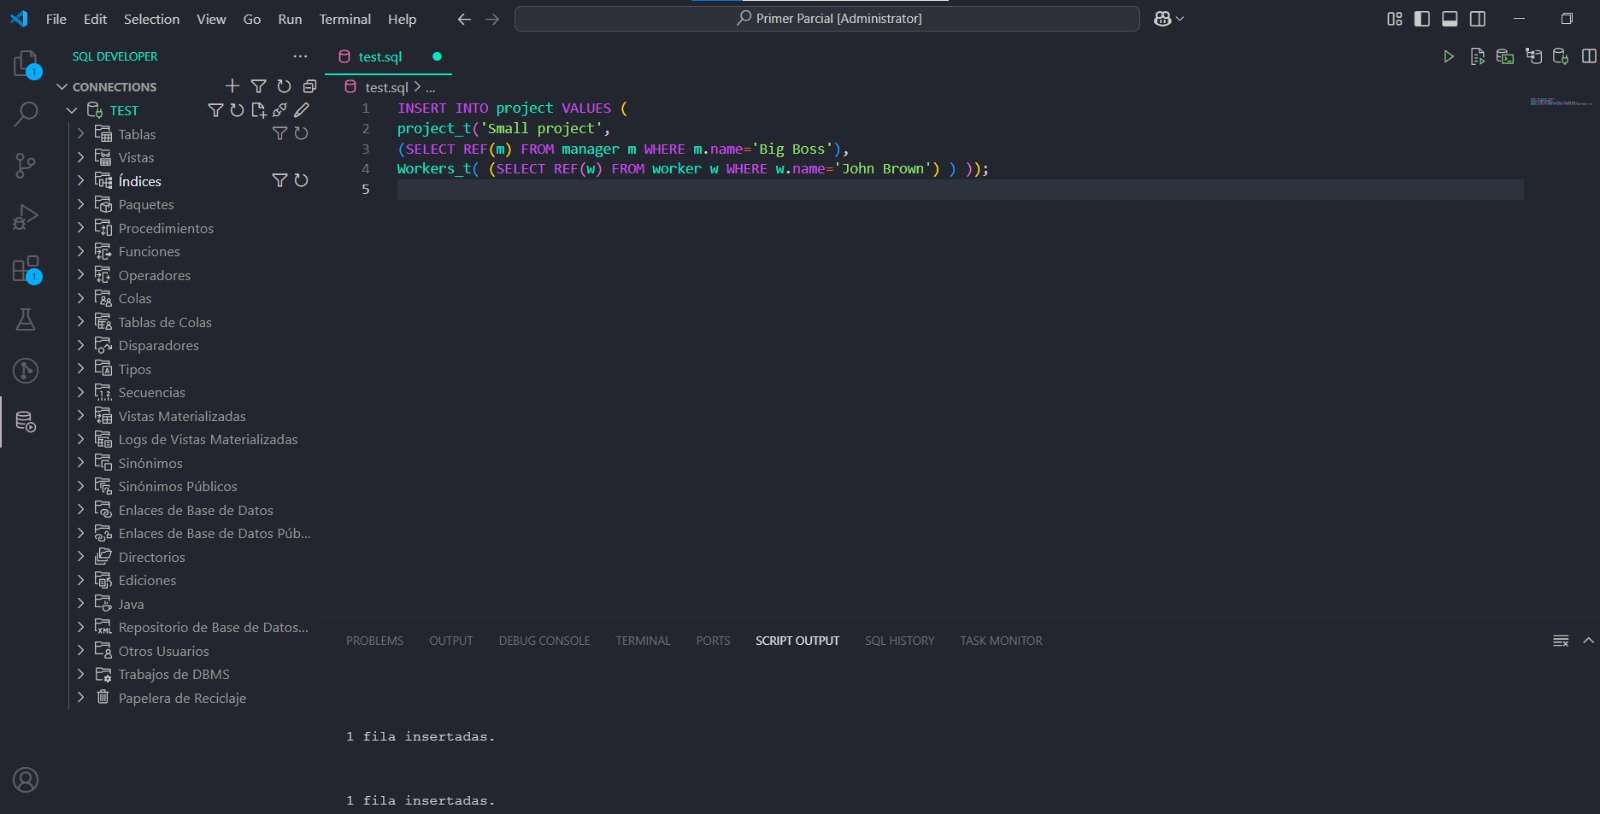
\includegraphics[width=1\textwidth]{imgs/inse4.jpeg}
	\caption{Insert query}
	\label{fig:12}
\end{figure}

\begin{figure}[H]
	\centering
	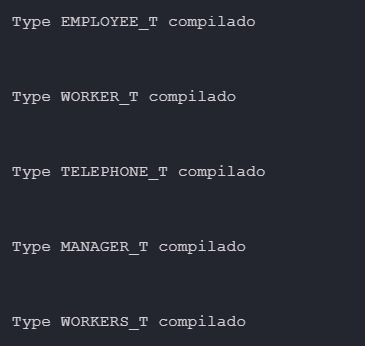
\includegraphics[width=1\textwidth]{imgs/comp.jpeg}
	\caption{compilation successfully}
	\label{fig:13}
\end{figure}


\begin{figure}[H]
	\centering
	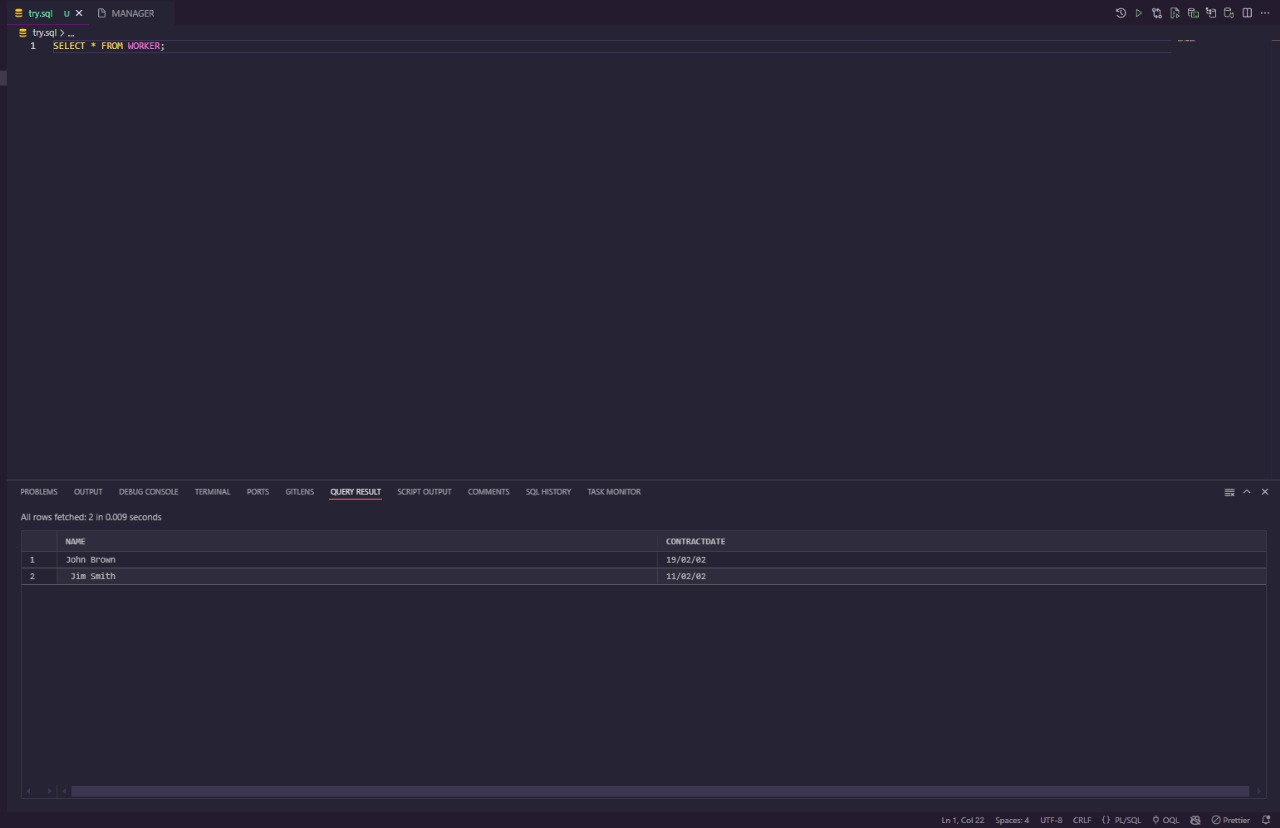
\includegraphics[width=1\textwidth]{imgs/sel1.jpeg}
	\caption{Select query}
	\label{fig:14}
\end{figure}

\begin{figure}[H]
	\centering
	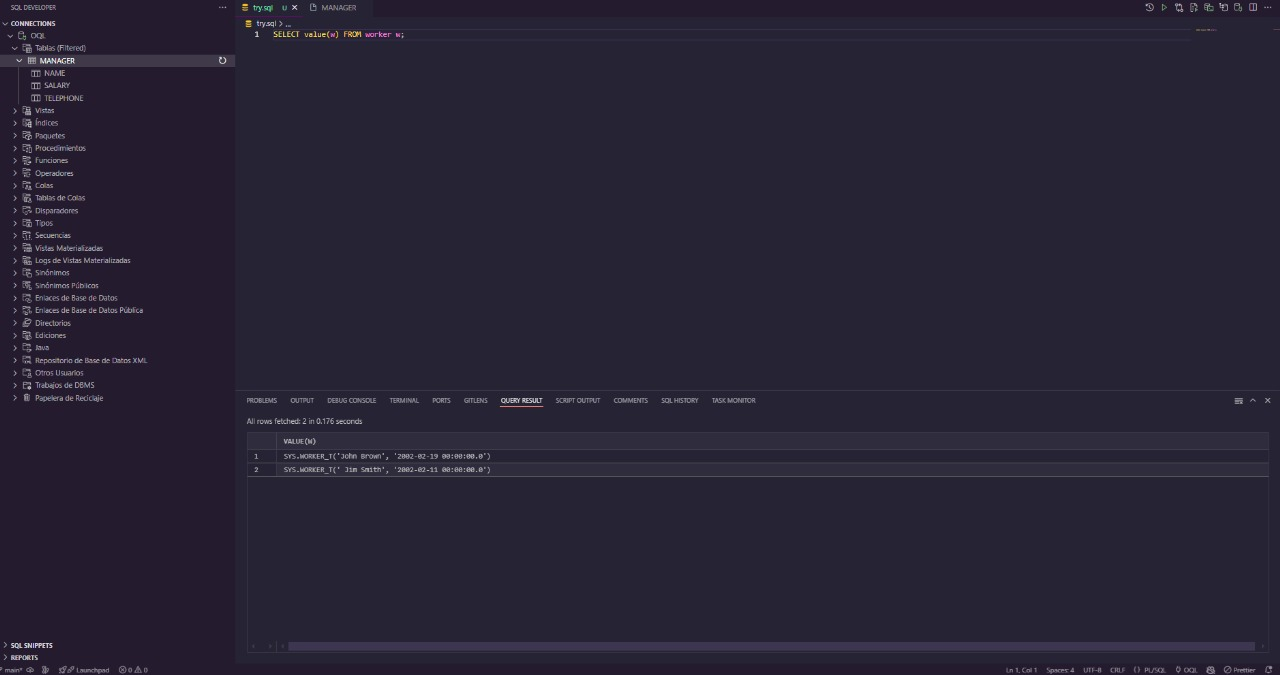
\includegraphics[width=1\textwidth]{imgs/sel2.jpeg}
	\caption{Select query}
	\label{fig:15}
\end{figure}

\begin{figure}[H]
	\centering
	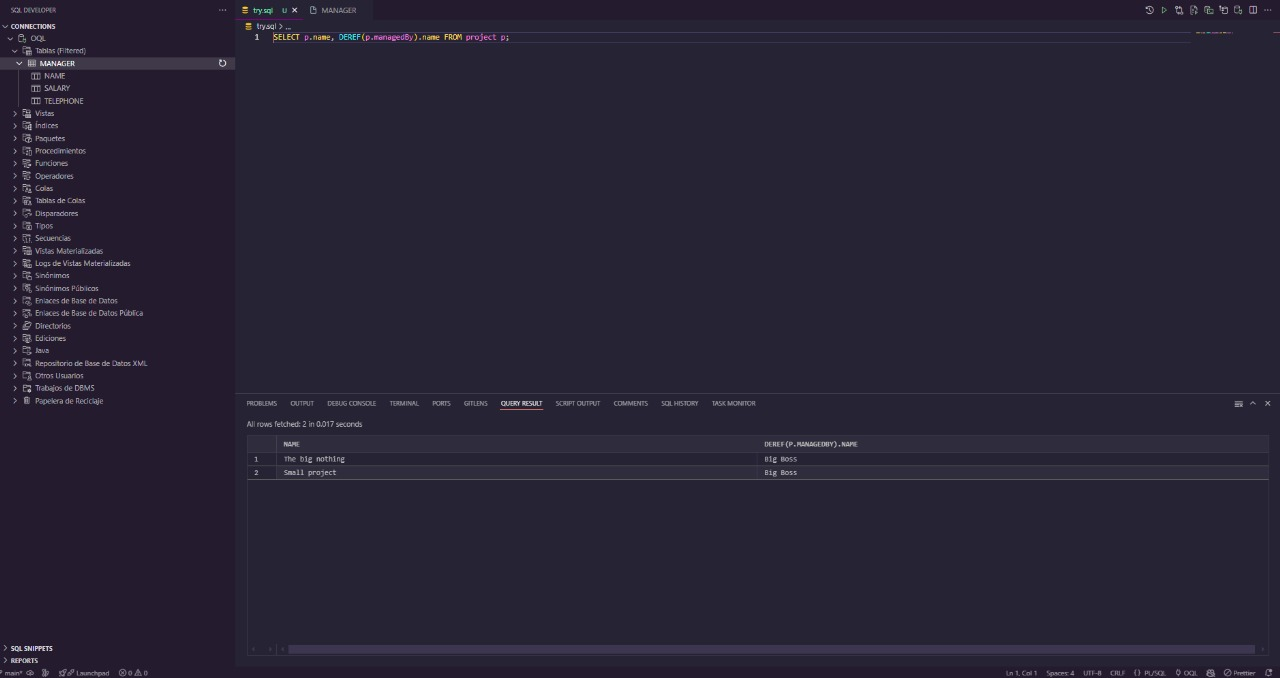
\includegraphics[width=1\textwidth]{imgs/sel3.jpeg}
	\caption{Select query}
	\label{fig:16}
\end{figure}

\begin{figure}[H]
	\centering
	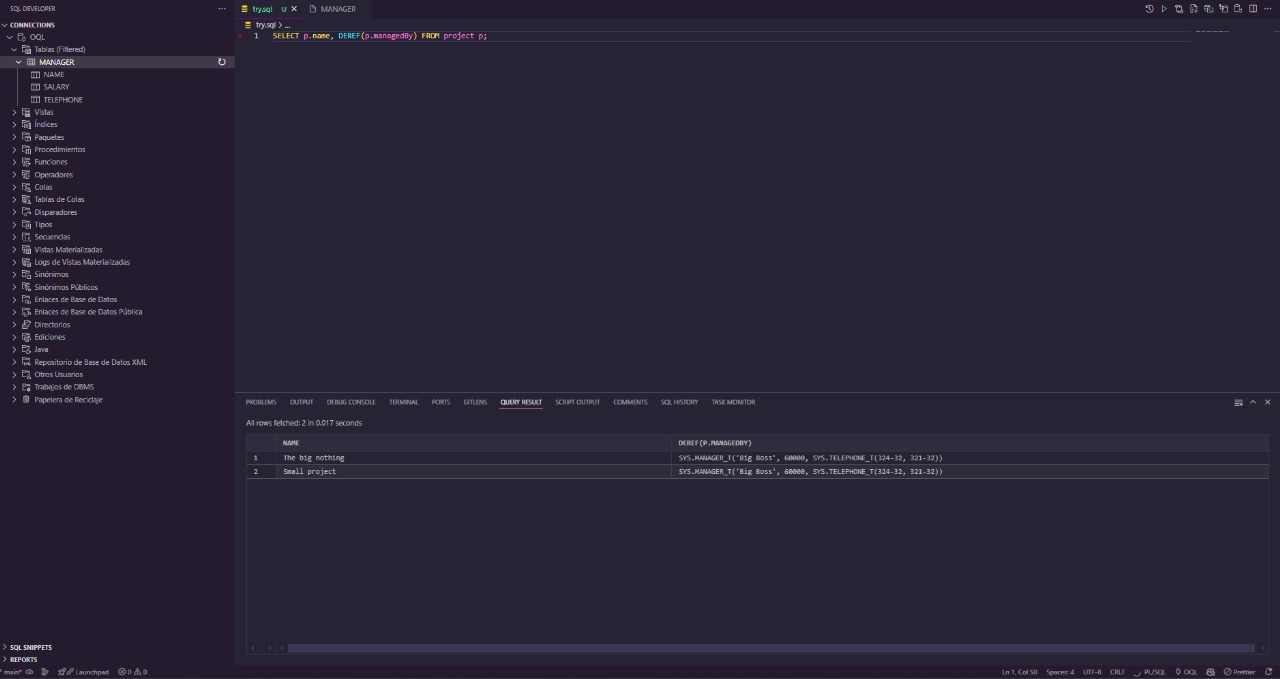
\includegraphics[width=1\textwidth]{imgs/sel4.jpeg}
	\caption{Select query}
	\label{fig:17}
\end{figure}

\begin{figure}[H]
	\centering
	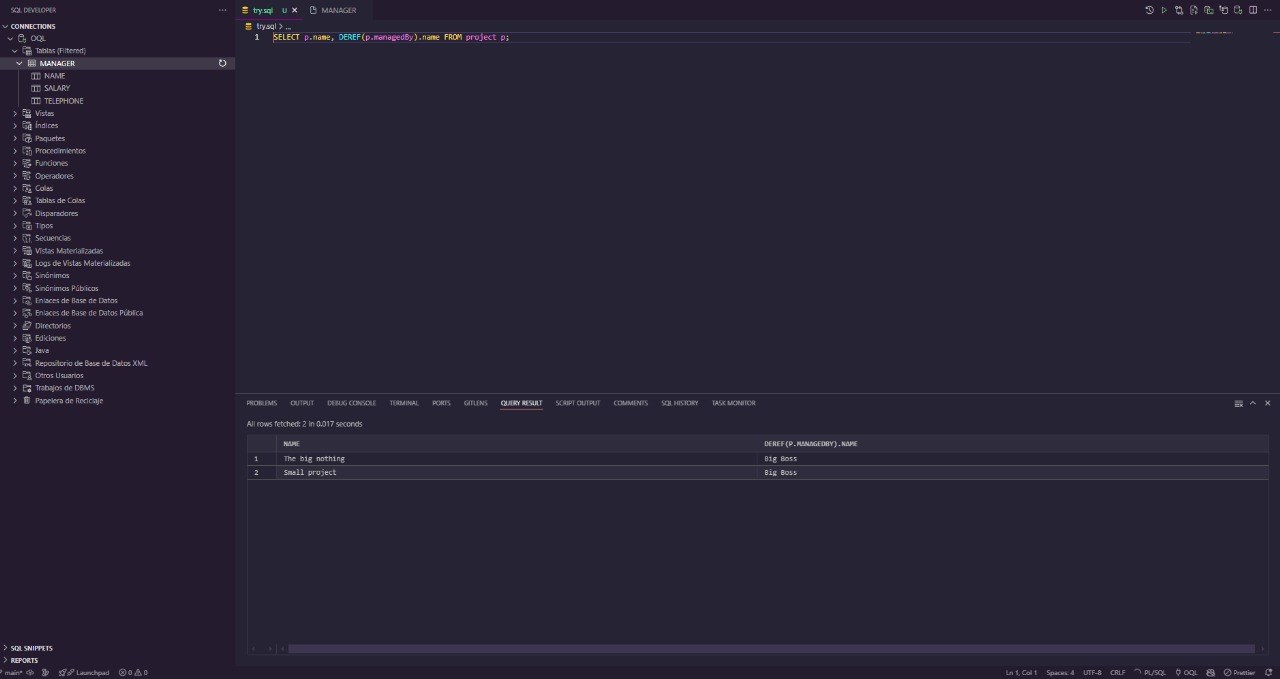
\includegraphics[width=1\textwidth]{imgs/sel5.jpeg}
	\caption{Select query}
	\label{fig:18}
\end{figure}

\begin{figure}[H]
	\centering
	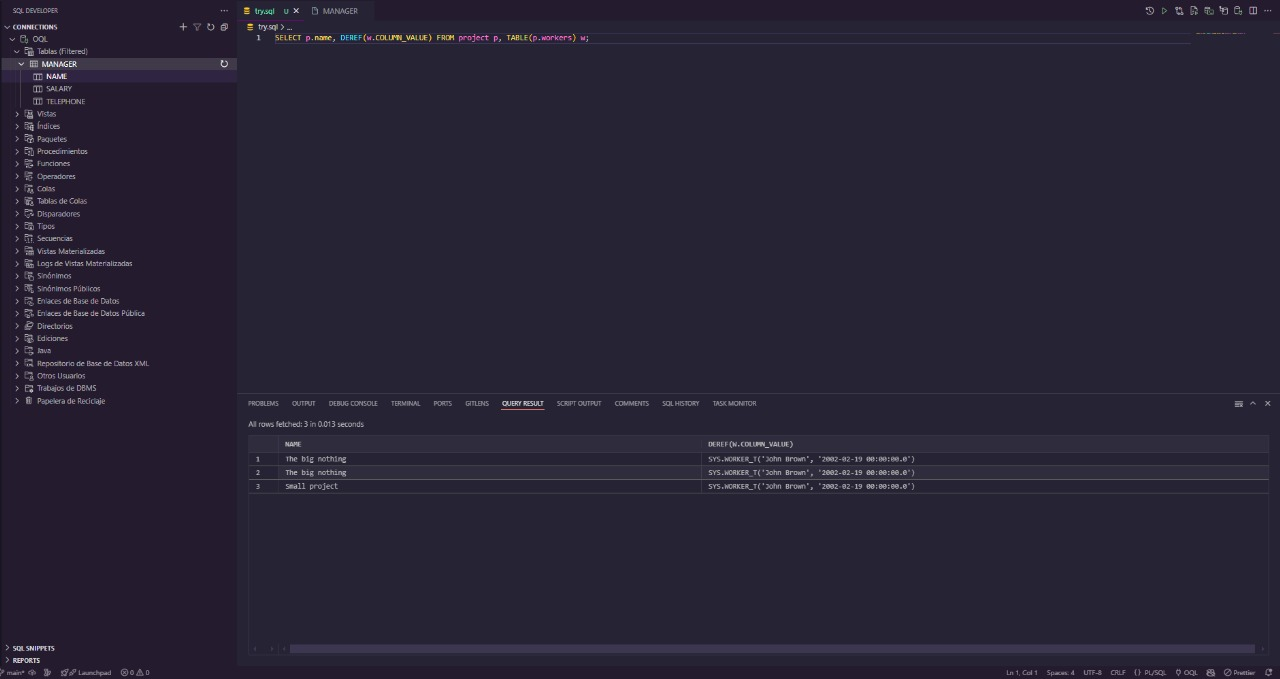
\includegraphics[width=1\textwidth]{imgs/sel6.jpeg}
	\caption{Select query}
	\label{fig:19}
\end{figure}

\subsection*{Summary of Results}
After overcoming the initial challenges of setting up the environment and configuring the Oracle extension in VSCode, we successfully executed the OQL scripts. The object types, tables, and relationships were created as expected, and the database schema was validated through a series of queries. The successful compilation and execution of the OQL scripts, as shown in the figures, demonstrate the effectiveness of OQL in managing object-relational databases. This exercise highlights the potential of OQL for modern, object-oriented applications, despite the initial difficulties encountered due to limited documentation.

\section{Conclusions}
This work demonstrated the effectiveness of Object Query Language (OQL) in managing object-relational databases. \textbf{However we as a team struggled a ton to get this tools working due to the lack of documentation that is online.} By defining complex object types, nested collections, and relationships, we showed that OQL simplifies querying object-oriented data compared to SQL, which relies on complex joins. OQL's native support for object-oriented principles, such as inheritance and polymorphism, makes it a superior choice for modern applications. This highlights OQL's potential for advancing database technologies in object-oriented contexts.

\section{EXTRA}

To implement the object-relational database system on an \textbf{any Linux} system, we used \textbf{Docker} to containerize the Oracle Database Express Edition (XE). This approach simplifies the setup process and ensures consistency across different environments. Below are the steps to run the system and execute the OQL scripts:

\subsection*{1. Start the Oracle XE Container}
First, start the Oracle XE container using the following command:
\begin{verbatim}
sudo docker start oracle-xe
\end{verbatim}

If the container does not exist, create it using:
\begin{verbatim}
sudo docker run -d \
  -p 1521:1521 \
  --name oracle-xe \
  -e ORACLE_PASSWORD=<Password> \
  -v /home/erick/SQLSexyQueries/oql:/sql \
  gvenzl/oracle-xe
\end{verbatim}
\begin{itemize}
    \item Replace \texttt{<Password>} with your desired password for the Oracle database.
    \item The \texttt{-v} flag mounts the local directory \texttt{/home/erick/SQLSexyQueries/oql} to the \texttt{/sql} directory inside the container, allowing you to access your SQL scripts.
\end{itemize}

\subsection*{2. Connect to the Oracle Database}
Once the container is running, connect to the Oracle database using \texttt{sqlplus}:
\begin{verbatim}
sqlplus sys/<Password>@//localhost:1521/XE as sysdba
\end{verbatim}
\begin{itemize}
    \item Replace \texttt{<Password>} with the password you set during container creation.
\end{itemize}

\subsection*{3. Execute the OQL Script}
To execute the OQL script (\texttt{t2.sql}) stored in the mounted directory, use the following command:
\begin{verbatim}
sudo docker exec -i oracle-xe sqlplus sys/<Password> as sysdba @/sql/t2.sql
\end{verbatim}
\begin{itemize}
    \item This command runs the \texttt{t2.sql} script inside the Oracle XE container.
\end{itemize}

\subsection*{4. OQL Script Overview}
The OQL script performs the following steps:
\begin{enumerate}
    \item \textbf{Clean Up Existing Objects}: Drops any existing tables or types to avoid conflicts.
    \item \textbf{Create Object Types}: Defines object types such as \texttt{employee\_t}, \texttt{worker\_t}, and \texttt{manager\_t} with attributes and methods.
    \item \textbf{Create Tables}: Creates tables with nested collections (e.g., \texttt{telephone\_t} as a nested table of phone numbers).
    \item \textbf{Insert Sample Data}: Populates the tables with sample data to demonstrate the functionality of the object-relational schema.
    \item \textbf{Query Data}: Executes queries to retrieve and validate the data, ensuring the schema works as expected.
\end{enumerate}

\subsection*{5. Example Queries}
The script includes queries to:
\begin{itemize}
    \item Retrieve all workers:
    \begin{verbatim}
    SELECT * FROM worker;
    \end{verbatim}
    \item Retrieve all managers:
    \begin{verbatim}
    SELECT * FROM manager;
    \end{verbatim}
    \item Retrieve all projects with their associated workers and managers:
    \begin{verbatim}
    SELECT p.name, DEREF(p.managedBy).name, DEREF(w.COLUMN_VALUE).name
    FROM project p, TABLE(p.workers) w;
    \end{verbatim}
\end{itemize}

\subsection*{6. Benefits of Using Docker}
\begin{itemize}
    \item \textbf{Isolation}: Docker ensures that the Oracle database runs in an isolated environment, avoiding conflicts with other software on the system.
    \item \textbf{Portability}: The containerized setup can be easily replicated on other systems, ensuring consistency across development and production environments.
    \item \textbf{Ease of Setup}: Docker simplifies the installation and configuration of Oracle Database XE, especially on Linux distributions like Arch Linux where manual installation can be complex.
\end{itemize}

By following these steps, you can successfully run the object-relational database system on any Linux using Docker and Oracle XE, and execute the OQL scripts to validate the schema.

\subsection*{PROVE}
The following SQL/OQL code was used to implement the object-relational database system:

\begin{verbatim}
-- Step 1: Clean up existing objects (if they exist)
BEGIN
  EXECUTE IMMEDIATE 'DROP TABLE project CASCADE CONSTRAINTS';
EXCEPTION
  WHEN OTHERS THEN
    IF SQLCODE != -942 THEN
      RAISE;
    END IF;
END;
/
BEGIN
  EXECUTE IMMEDIATE 'DROP TABLE manager CASCADE CONSTRAINTS';
EXCEPTION
  WHEN OTHERS THEN
    IF SQLCODE != -942 THEN
      RAISE;
    END IF;
END;
/
BEGIN
  EXECUTE IMMEDIATE 'DROP TABLE worker CASCADE CONSTRAINTS';
EXCEPTION
  WHEN OTHERS THEN
    IF SQLCODE != -942 THEN
      RAISE;
    END IF;
END;
/
BEGIN
  EXECUTE IMMEDIATE 'DROP TYPE project_t FORCE';
EXCEPTION
  WHEN OTHERS THEN
    IF SQLCODE != -4043 THEN
      RAISE;
    END IF;
END;
/
BEGIN
  EXECUTE IMMEDIATE 'DROP TYPE workers_t FORCE';
EXCEPTION
  WHEN OTHERS THEN
    IF SQLCODE != -4043 THEN
      RAISE;
    END IF;
END;
/
BEGIN
  EXECUTE IMMEDIATE 'DROP TYPE manager_t FORCE';
EXCEPTION
  WHEN OTHERS THEN
    IF SQLCODE != -4043 THEN
      RAISE;
    END IF;
END;
/
BEGIN
  EXECUTE IMMEDIATE 'DROP TYPE telephone_t FORCE';
EXCEPTION
  WHEN OTHERS THEN
    IF SQLCODE != -4043 THEN
      RAISE;
    END IF;
END;
/
BEGIN
  EXECUTE IMMEDIATE 'DROP TYPE worker_t FORCE';
EXCEPTION
  WHEN OTHERS THEN
    IF SQLCODE != -4043 THEN
      RAISE;
    END IF;
END;
/
BEGIN
  EXECUTE IMMEDIATE 'DROP TYPE employee_t FORCE';
EXCEPTION
  WHEN OTHERS THEN
    IF SQLCODE != -4043 THEN
      RAISE;
    END IF;
END;
/

-- Step 2: Create object types
CREATE TYPE employee_t AS OBJECT (name varchar2(100)) NOT FINAL;
/
CREATE TYPE worker_t UNDER employee_t (contractDate date);
/
CREATE TYPE telephone_t AS TABLE OF varchar2(30);
/
CREATE TYPE manager_t UNDER employee_t (salary integer, telephone telephone_t);
/
CREATE TYPE workers_t AS TABLE OF REF worker_t;
/
CREATE TYPE project_t AS OBJECT (
  name varchar2(100),
  managedBy REF manager_t,
  workers workers_t
);
/

-- Step 3: Create tables
CREATE TABLE worker OF worker_t;
CREATE TABLE manager OF manager_t NESTED TABLE telephone STORE AS telephone_nt;
CREATE TABLE project OF project_t NESTED TABLE workers STORE AS workers_nt;

-- Step 4: Add constraints
ALTER TABLE project ADD (SCOPE FOR (managedBy) IS manager);
ALTER TABLE workers_nt ADD (SCOPE FOR (COLUMN_VALUE) IS worker);

-- Step 5: Insert sample data
-- Insert workers
INSERT INTO worker VALUES ('John Brown', TO_DATE('19-FEB-2002', 'DD-MON-YYYY'));
INSERT INTO worker VALUES (worker_t('Jim Smith', TO_DATE('11-FEB-2002', 'DD-MON-YYYY')));

-- Insert manager
INSERT INTO manager VALUES (
  manager_t('Big Boss', 60000, telephone_t('324-32', '321-32'))
);

-- Insert project with no workers
INSERT INTO project VALUES (
  'The big nothing',
  (SELECT REF(m) FROM manager m WHERE m.name='Big Boss'),
  workers_t()
);

-- Assign workers to the project
INSERT INTO TABLE (
  SELECT workers FROM project WHERE name='The big nothing'
) (
  SELECT REF(w) FROM worker w WHERE w.name='John Brown' OR w.name='Jim Smith'
);

-- Insert another project with one worker
INSERT INTO project VALUES (
  project_t(
    'Small project',
    (SELECT REF(m) FROM manager m WHERE m.name='Big Boss'),
    workers_t((SELECT REF(w) FROM worker w WHERE w.name='John Brown'))
  )
);

-- Step 6: Verify data
-- Query all workers
SELECT * FROM worker;
-- Query all managers
SELECT * FROM manager;
-- Query all projects
SELECT p.name, DEREF(p.managedBy).name, DEREF(w.COLUMN_VALUE).name
FROM project p, TABLE(p.workers) w;
\end{verbatim}

This implementation demonstrates the key features of object-relational databases using OQL:

\begin{enumerate}
    \item Object type hierarchy with \texttt{employee\_t} as the base type and \texttt{worker\_t} and \texttt{manager\_t} as derived types
    \item Nested collections using \texttt{telephone\_t} for manager phone numbers
    \item Object references with \texttt{REF manager\_t} and \texttt{workers\_t}
    \item Complex queries using \texttt{DEREF} to access referenced objects
\end{enumerate}

The successful execution of these queries, as shown in the previous figures, validates the correct implementation of our object-relational schema.

\begin{figure}[H]
	\centering
	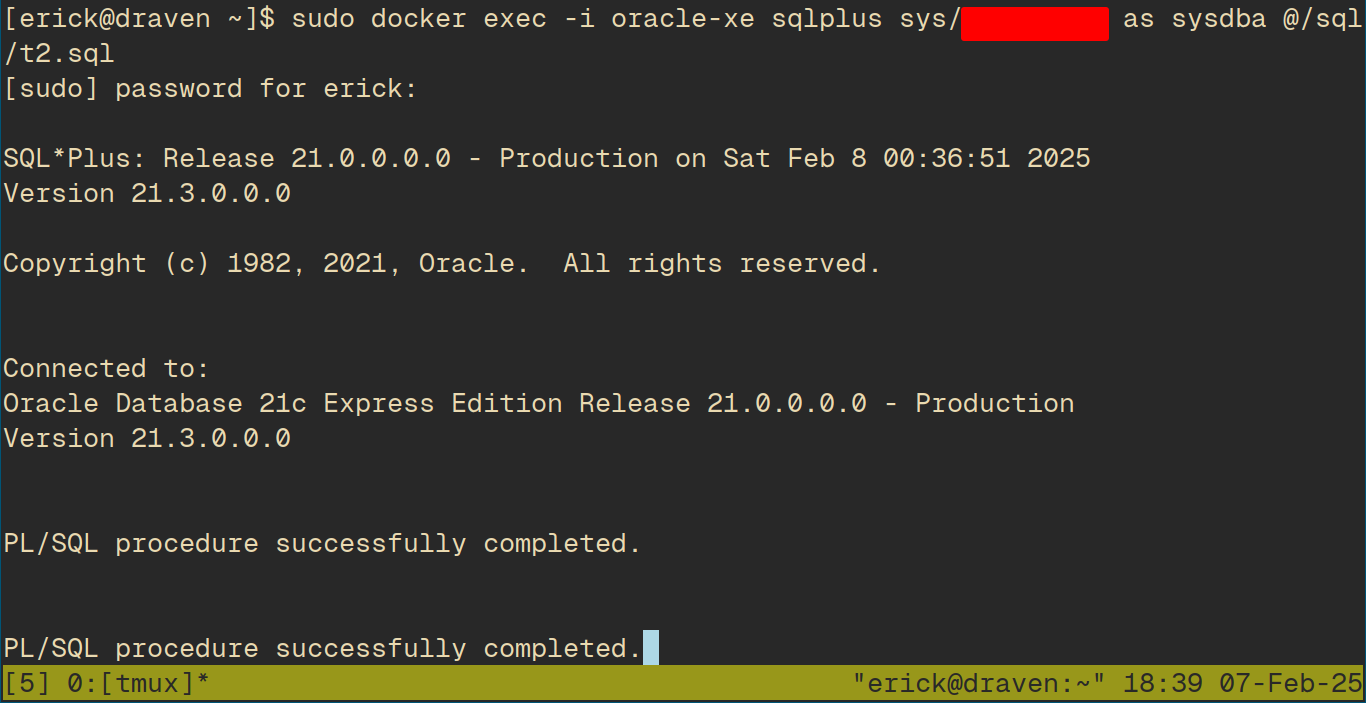
\includegraphics[width=1\textwidth]{imgs/p1.png}
	\caption{Successfull compilation}
	\label{fig:20}
\end{figure}

\begin{figure}[H]
	\centering
	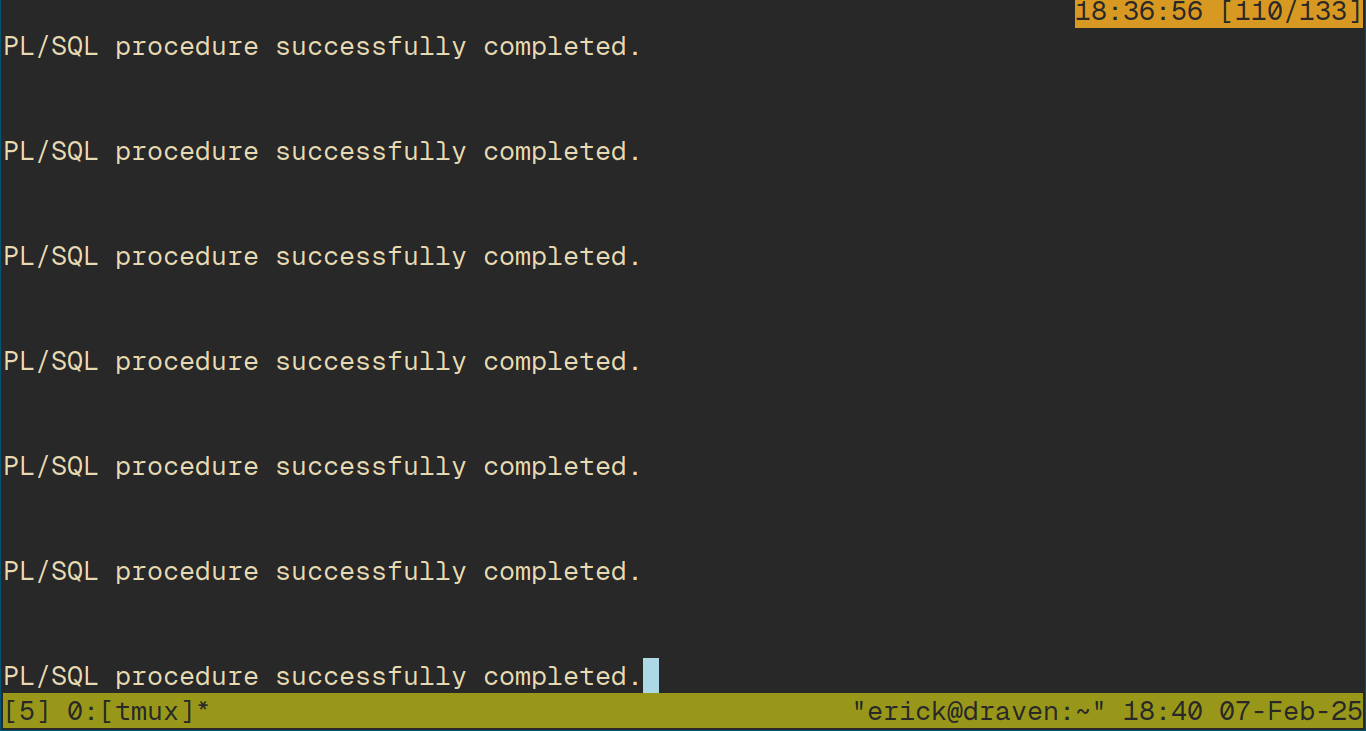
\includegraphics[width=1\textwidth]{imgs/p2.png}
	\caption{Successfull compilation}
	\label{fig:21}
\end{figure}

\begin{figure}[H]
	\centering
	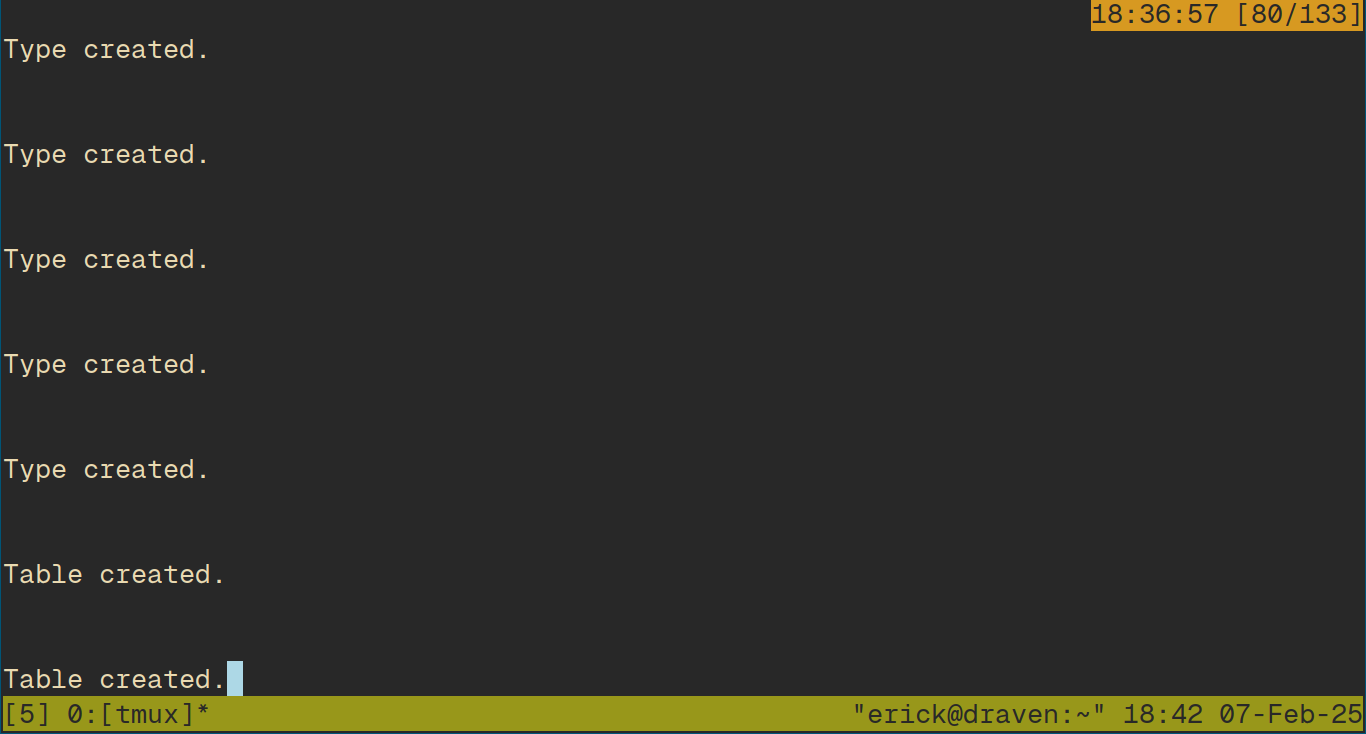
\includegraphics[width=1\textwidth]{imgs/p3.png}
	\caption{Successfull compilation}
	\label{fig:22}
\end{figure}

\begin{figure}[H]
	\centering
	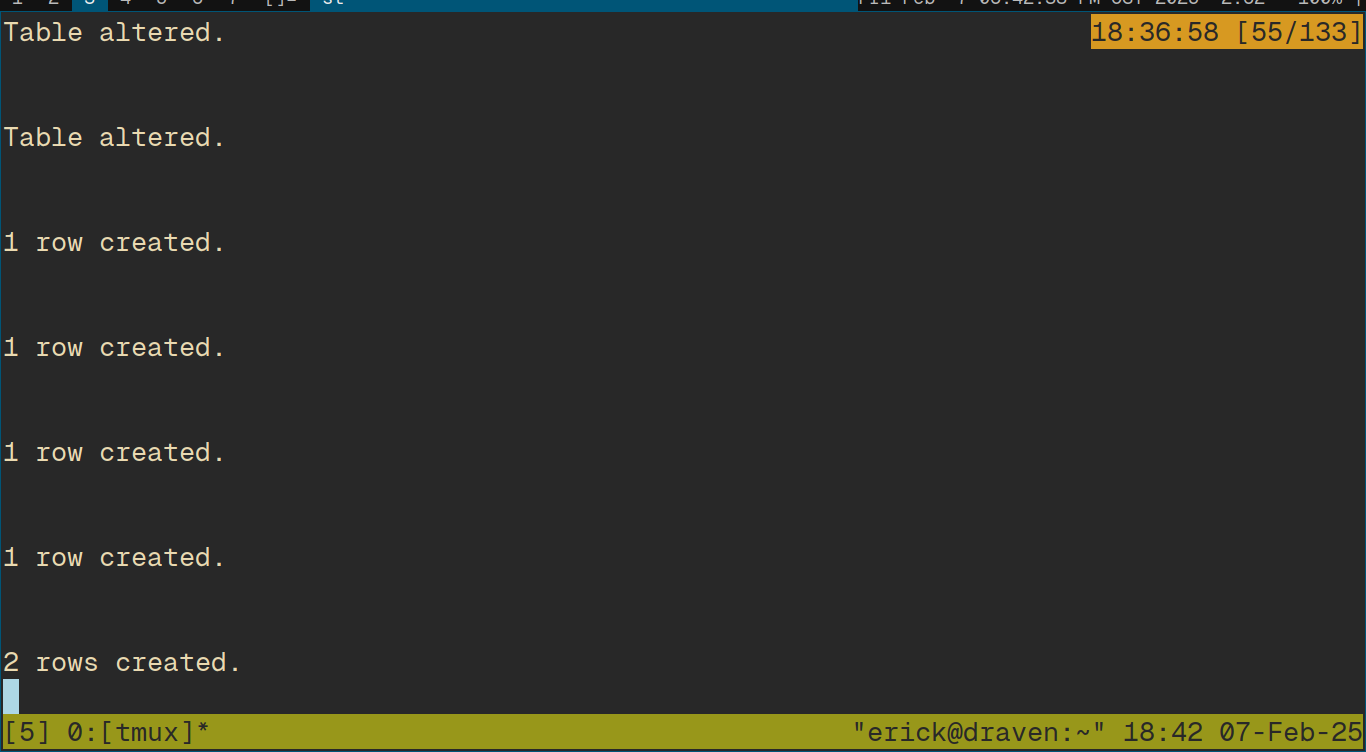
\includegraphics[width=1\textwidth]{imgs/p4.png}
	\caption{Successfull compilation}
	\label{fig:23}
\end{figure}


\begin{figure}[H]
	\centering
	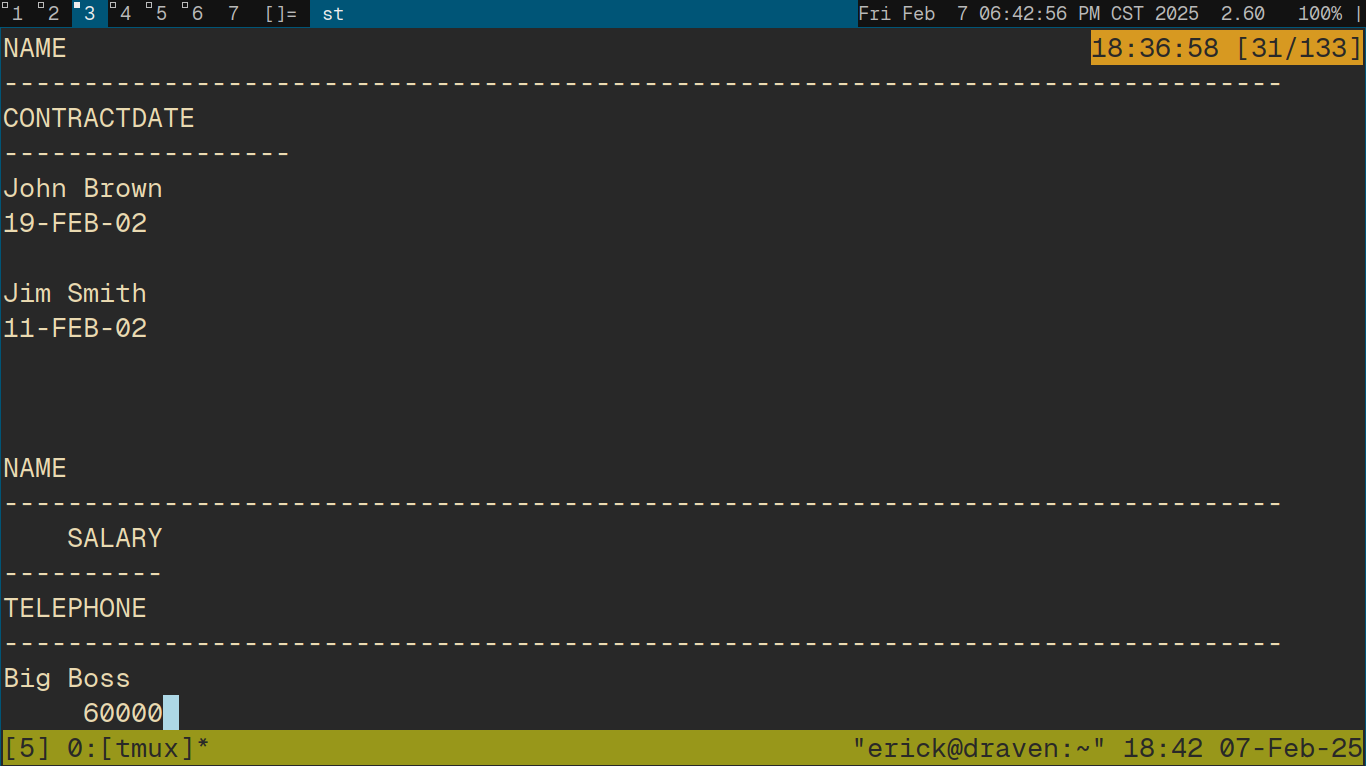
\includegraphics[width=1\textwidth]{imgs/p5.png}
	\caption{Successfull compilation}
	\label{fig:24}
\end{figure}


\begin{figure}[H]
	\centering
	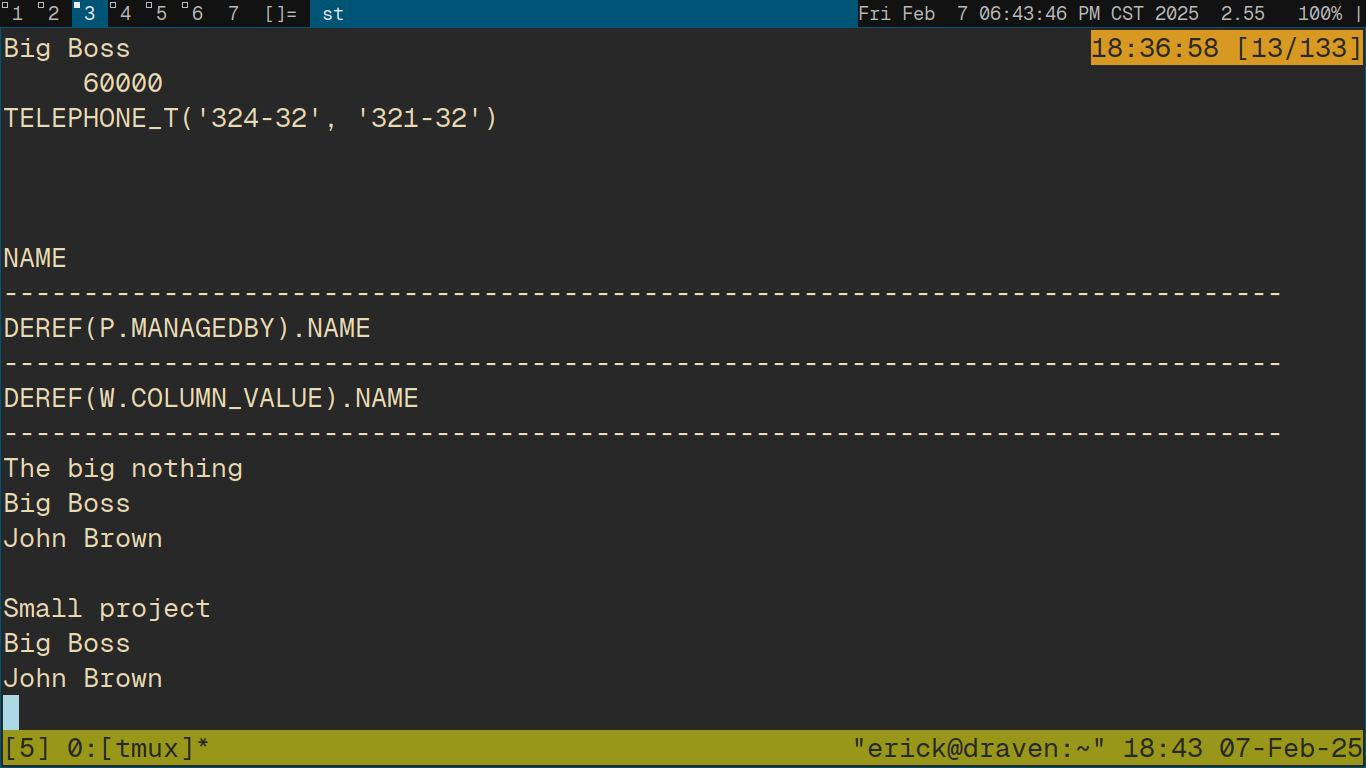
\includegraphics[width=1\textwidth]{imgs/p6.png}
	\caption{The queries}
	\label{fig:25}
\end{figure}

\begin{figure}[H]
	\centering
	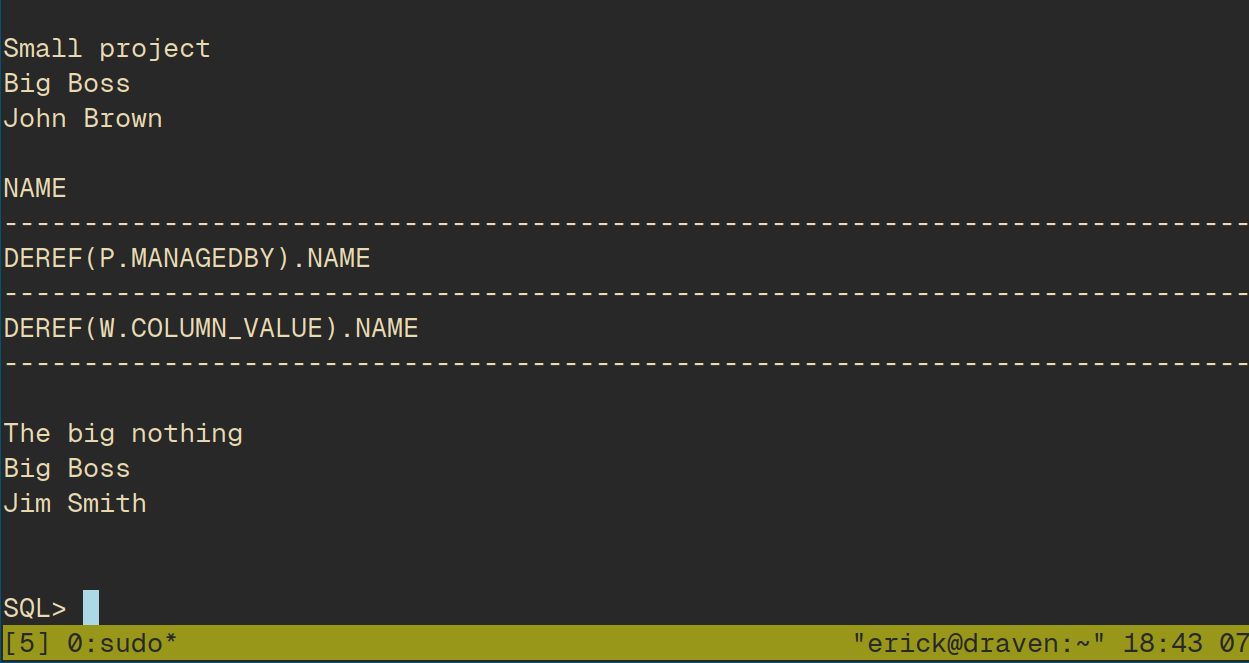
\includegraphics[width=1\textwidth]{imgs/p7.png}
	\caption{The queries}
	\label{fig:26}
\end{figure}

\begin{thebibliography}{9}
	\bibitem{mendix}
	OQL. (n.d.). Mendix Documentation. Retrieved February 7, 2025, from https://docs.mendix.com/refguide/oql/
	\bibitem{ibm}
	Tivoli Network Manager IP edition 4.2.0. (2025, January 21). Ibm.com. https://www.ibm.com/docs/en/networkmanager/4.2.0?topic=reference-object-query-language
	\bibitem{w3s}
	What is SQL. (n.d.). W3schools.com. Retrieved February 7, 2025, from https://www.w3schools.com/whatis/whatis\_sql.asp
\end{thebibliography}

\end{document}
